\newpage

\subsection{QuizziPedia::Front-End::Models}

	\label{QuizziPedia::Front-End::Models}
	
	\begin{figure}[h]
		\centering
		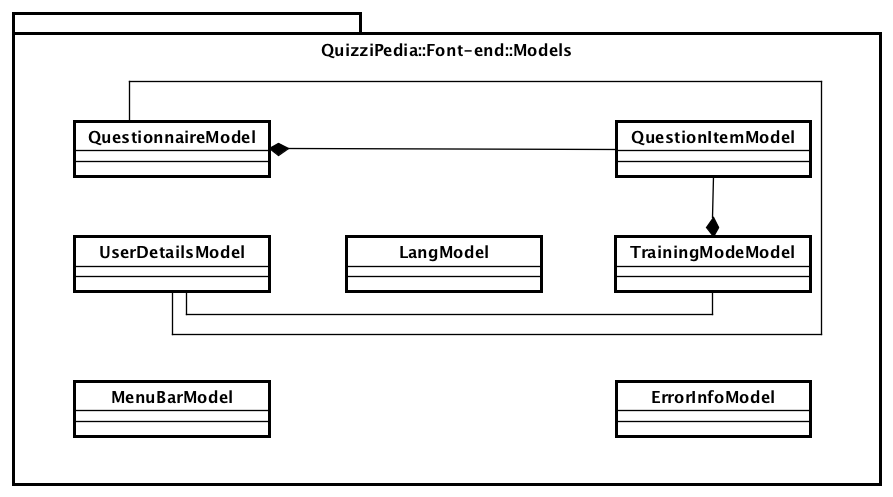
\includegraphics[scale=0.5,keepaspectratio]{UML/Package/QuizziPedia_Front-End_Models.png}
		\caption{QuizziPedia::Front-End::Models}
	\end{figure}

	\subsubsection{Informazioni generali}
		\begin{itemize}
			\item \textbf{Descrizione}: package contenente le classi che definiscono la business logic dell'applicazione;
			\item \textbf{Padre}: \texttt{Front-End};
			\item \textbf{Iterazioni con altri componenti}: 
				\begin{itemize}				
					\item \texttt{Controllers}: package contenente i controllers front-end dell'applicazione;
					\item \texttt{Directives}: package contenente le directives front-end dell'applicazione;
					\item \texttt{Models}: package contenente le classi che definiscono la business logic dell'applicazione;
					\item \texttt{Templates}: package contenente i templates necessari per la creazione dinamica delle viste per le domande;
					\item \texttt{Services}: package che contiene le classi individuate che permettono la comunicazione del lato front-end con il lato back-end attraverso l'architettura REST.
				\end{itemize}

		\end{itemize}
	
	\subsubsection{Classi}
		\paragraph{QuizziPedia::Front-End::Models::ErrorInfoModel}
		
		\label{QuizziPedia::Front-End::Models::ErrorInfoModel}
		
		\begin{figure}[h]
			\centering
			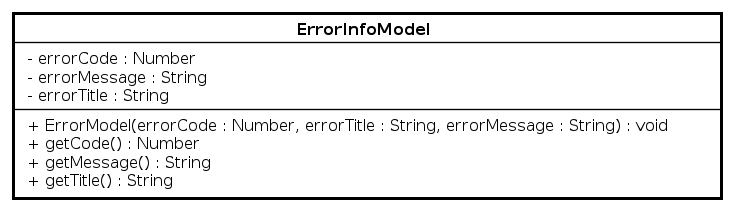
\includegraphics[scale=0.5,keepaspectratio]{UML/Classi/Front-End/QuizziPedia_Front-end_Models_ErrorInfoModel.png}
			\caption{QuizziPedia::Front-End::Models::ErrorInfoModel}
		\end{figure}
		
		\begin{itemize}
			\item \textbf{Descrizione}: ;
			\item \textbf{Utilizzo}: ;
			\item \textbf{Relazioni con altre classi}: 
			\begin{itemize}
				\item ;
			\end{itemize}
			\item \textbf{Attributi}: 
			\begin{itemize}
				\item ;
			\end{itemize}
			\item \textbf{Metodi}: 
			\begin{itemize}
				\item ;
			\end{itemize}
		\end{itemize}
			
		\paragraph{QuizziPedia::Front-End::Models::LangModel}
		
		\label{QuizziPedia::Front-End::Models::LangModel}
		
		\begin{figure}[h]
			\centering
			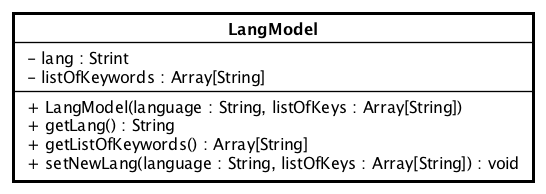
\includegraphics[scale=0.5,keepaspectratio]{UML/Classi/Front-End/QuizziPedia_Front-end_Models_LangModel.png}
			\caption{QuizziPedia::Front-End::Models::LangModel}
		\end{figure}
		
		\begin{itemize}
			\item \textbf{Descrizione}: ;
			\item \textbf{Utilizzo}: ;
			\item \textbf{Relazioni con altre classi}: 
			\begin{itemize}
				\item ;
			\end{itemize}
			\item \textbf{Attributi}: 
			\begin{itemize}
				\item ;
			\end{itemize}
			\item \textbf{Metodi}: 
			\begin{itemize}
				\item ;
			\end{itemize}
		\end{itemize}
		
		\paragraph{QuizziPedia::Front-End::Models::QuestionItemModel}
		
		\label{QuizziPedia::Front-End::Models::QuestionItemModel}
		
		\begin{figure}[h]
			\centering
			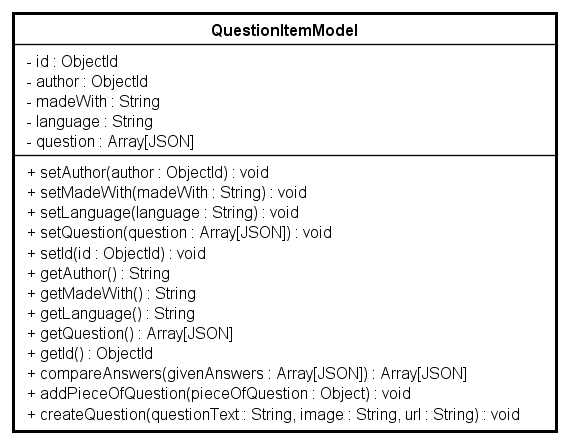
\includegraphics[scale=0.5,keepaspectratio]{UML/Classi/Front-End/QuizziPedia_Front-end_Models_QuestionItemModel.png}
			\caption{QuizziPedia::Front-End::Models::QuestionItemModel}
		\end{figure}
		
		\begin{itemize}
			\item \textbf{Descrizione}: ;
			\item \textbf{Utilizzo}: ;
			\item \textbf{Relazioni con altre classi}: 
			\begin{itemize}
				\item ;
			\end{itemize}
			\item \textbf{Attributi}: 
			\begin{itemize}
				\item ;
			\end{itemize}
			\item \textbf{Metodi}: 
			\begin{itemize}
				\item ;
			\end{itemize}
		\end{itemize}
		
		\paragraph{QuizziPedia::Front-End::Models::QuestionnaireModel}
		
		\label{QuizziPedia::Front-End::Models::QuestionnaireModel}
		
		\begin{figure}[h]
			\centering
			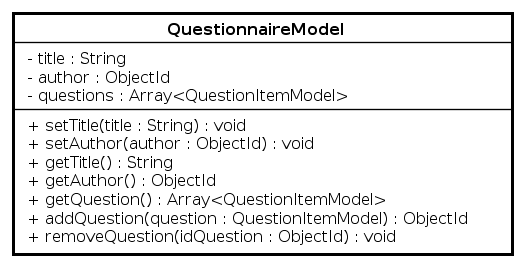
\includegraphics[scale=0.5,keepaspectratio]{UML/Classi/Front-End/QuizziPedia_Front-end_Models_QuestionnaireModel.png}
			\caption{QuizziPedia::Front-End::Models::QuestionnaireModel}
		\end{figure}
		
		\begin{itemize}
			\item \textbf{Descrizione}: ;
			\item \textbf{Utilizzo}: ;
			\item \textbf{Relazioni con altre classi}: 
			\begin{itemize}
				\item ;
			\end{itemize}
			\item \textbf{Attributi}: 
			\begin{itemize}
				\item ;
			\end{itemize}
			\item \textbf{Metodi}: 
			\begin{itemize}
				\item ;
			\end{itemize}
		\end{itemize}	
		
		\paragraph{QuizziPedia::Front-End::Models::TrainingModeModel}
		
		\label{QuizziPedia::Front-End::Models::TrainingModeModel}
		
		\begin{figure}[h]
			\centering
			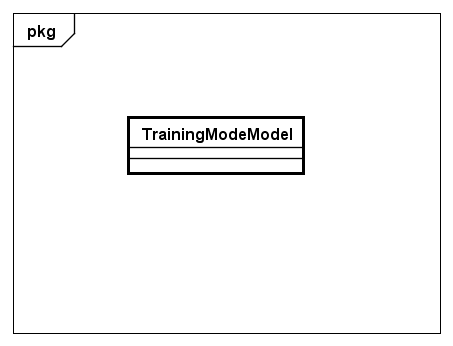
\includegraphics[scale=0.5,keepaspectratio]{UML/Classi/Front-End/QuizziPedia_Front-end_Models_TrainingModeModel.png}
			\caption{QuizziPedia::Front-End::Models::TrainingModeModel}
		\end{figure}
		
		\begin{itemize}
			\item \textbf{Descrizione}: ;
			\item \textbf{Utilizzo}: ;
			\item \textbf{Relazioni con altre classi}: 
			\begin{itemize}
				\item ;
			\end{itemize}
			\item \textbf{Attributi}: 
			\begin{itemize}
				\item ;
			\end{itemize}
			\item \textbf{Metodi}: 
			\begin{itemize}
				\item ;
			\end{itemize}
		\end{itemize}
			
		\paragraph{QuizziPedia::Front-End::Models::UserDetailsModel}
		
		\label{QuizziPedia::Front-End::Models:.UserDetailsModel}
		
		\begin{figure}[h]
			\centering
			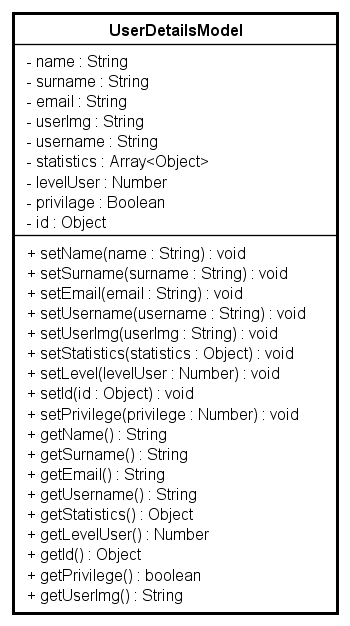
\includegraphics[scale=0.5,keepaspectratio]{UML/Classi/Front-End/QuizziPedia_Front-end_Models_UserDetailsModel.png}
			\caption{QuizziPedia::Front-End::Models::UserDetailsModel}
		\end{figure}
		
		\begin{itemize}
			\item \textbf{Descrizione}: ;
			\item \textbf{Utilizzo}: ;
			\item \textbf{Relazioni con altre classi}: 
			\begin{itemize}
				\item ;
			\end{itemize}
			\item \textbf{Attributi}: 
			\begin{itemize}
				\item ;
			\end{itemize}
			\item \textbf{Metodi}: 
			\begin{itemize}
				\item ;
			\end{itemize}
		\end{itemize}													